%*****************************************
\chapter{Literature Review}\label{ch:litreview}
%*****************************************
%todo: find relevant and insightful papers on the topic. FIN

%Hybrid heat pump can also refer to a dual energy input heat up. Find way to exclude this from search term. On google scholar, -"blahblah" can be used. Not sure if the same is true on OneSearch. 

% Very vert briefly explain how heat transfer work w.r.t. heating/cooling houses. Briefly explain heat pumps, some equations. Explain what a bivalent heat pump system is, will not be too commonly known. 
% Introduce relevant papers. What did they find, what did they do.

The literature review chapter provides a comprehensive overview of the relevant literature in the field of HHSs, including \HPs, \acp{HDD}, \ac{PE}, electrification of heating, controllers and control theory, and verification and validation of models. In particular, \cref{sec:heatpumps} focuses on \HPs, covering the vapour-compression cycle, \acp{HHS}, bivalent operating modes, buffer tanks, frosting and defrosting. \cref{sec:hddanddesign} examines \acp{HDD} and design temperatures, while \cref{sec:primaryenergy} discusses into \ac{PE} considerations. \cref{sec:elecheating} discusses the electrification of heating, and section \cref{sec:controltheory} discusses controllers and basic control theory, including \ac{PID} controllers, noise, and error. Finally, \cref{sec:verifyandvalid} examines the verification and validation of the model, including validation techniques, methodologies, statistical indices and their associated tolerances.

\section{Heat Pumps} \label{sec:heatpumps}
\acp{HP} work by harnessing the energy from low temperature sources such as air, water or the ground. \HPs of any kind acquire energy from its surrounding environment in the form of low-temperature heat and \textit{concentrate} it to heat comparatively minute volumes to its surroundings. This is achieved through a vapour compression cycle, explained in \cref{subsec:vapourcompcycle}. Under ideal conditions, \acp{AWHP} have extremely high \acp{COP} in the \num{3.5} to \num{4.5} range. This is of course from their ability to harvest the aerothermal energy from the outside air. The main downfall of \acp{AWHP} is that when the external air temperature is low, their \ac{COP} is reduced significantly. Due to this inherent disadvantage, \acp{HP} are essentially unfit be the sole space heating generator for almost all applications, depending on climates and design points. While \HPs have the capacity to perform heating and cooling, this thesis and associated simulations do not consider the cooling of a building or home, and therefore is only concerned with heating and considers only the heating-season time frame of the year. The space-heating radiators found in existing homes are not suitable for cooling \cite{klein_numerical_2014}, the cold water in the radiators does not warm the room effectively and condensation on the radiator surface may become and issue. 

Because the efficiency of \acp{HP} is so dependent on the constantly varying outside air temperature, the measure of \ac{SPF} is typically used to characterise them when considering the performance over a certain heating period and is considered a more comprehensive metric to establish \HP efficiency \cite{seai_heat_2020,nowak_2018}. The \ac{SPF} represents the ratio of the total useful energy produced by the \ac{HP} during a heating season, to the seasonal electricity consumption. For example, an \ac{SPF} of 3 would mean that over a given year, the \ac{HP} produced 3 units of heating energy for every unit of electrical energy provided \cite{seai_heat_2020}. Due to \acp{HP} extracting renewable energy from the surrounding air, the \ac{SPF} is (or should be) always higher than 1, and generally is above 3. EU legislation states that in order to be eligible for the \ac{RHI}, the \ac{SPF} of a \ac{HP} must be above 2.5 \cite{eu-114-2014}. 

There are three main types of \acp{HP} for space heating (i.e., not air-conditioning): \acp{AWHP}, Ground-Water Heat Pumps and Hydro-Water Heat Pumps \cite{omer_2008,Ochsner_2007}. Ground-Water \acp{HP} acquire their heat energy by exploiting the heat contained within the soil of the Earth. Soil, below a certain depth has a very consistent heat, only fluctuating mildly seasonally. The added benefit of this type is that soil below a certain depth will not freeze, which would cause frosting like in \acp{AWHP}. Hydro-Water \acp{HP} gain their heat from water sources such as ponds, lakes or well-water. The temperature of water fluctuates far less than the ambient air temperature, meaning they do not extract as much energy as \acp{AWHP} on warmer days, however, during warmer days, the heating load of a residential home is much less than the peak load. Conversely, during very cold days, the water remains much warmer than the air, which is very beneficial during those high-load spells. These two types of \acp{HP}, due to their heat sources, have their merits, however, it is also due to their heat sources that they are relatively obscure and not commonplace. Installing these types of \acp{HP} is costly, complicated, time consuming and require permits to build. Due to these reasons, \acp{AWHP} are the most common form of \ac{HP} sold in Europe \cite{ehpa_2015}.  

\acp{HP} come in many different heat capacities, from single kilo-watt units to extremely large units which can heat large multi storey office buildings. In residential home contexts, the largest \acp{HP} generally available are almost \SI{300}{\kilo\watt}, but usually fall in around the \qtyrange{5}{20}{\kilo\watt} range. If an \ac{ASHP} were to be sized so large as to have the capacity to provide the entire heating envelope of a residential home during even the coldest expected temperatures, the \ac{ASHP} would (aside from being prohibitively expensive), be so oversized that when temperatures are moderate, the \ac{HP} would produce so much heat as to heat the space so quickly that it would have an extremely short on-off cycle \cite{bee_air-source_2019}. Since the peak load for heating occurs for a very small number of hours during any given heating period, this would be very detrimental to the unit, specifically the condenser component. The frequent on-off cycling significantly reduces the longevity of the condenser, and would require replacement long before what would be expected \cite{STIEBEL_2012}. Many manufacturers suggest that the number of on-off cycles should not exceed 6 per hour. %FIND SOURCE
To avoid this issue, \acp{AWHP} are specifically undersized. Various ``design temperatures'' can be calculated for a given location. For Dublin, the design temperature which covers 99.0\% of the annual heating is \SI{-0.7}{\celsius}. \acp{AWHP} are usually sized to meet a design temperature of 60\%--70\%, as opposed to more traditional space heaters, as is further explained in \cref{sec:hddanddesign}.

\acp{HP} tend to perform better when providing space heating through underfloor heating \cite{seai_heat_2020}. This is partly due to underfloor heating being more efficient in general than other, more traditional space heating methods, namely hot-water radiators. Another reason more applicable to \acp{HP} is that the (space heating) inlet water temperature for underfloor heating is much lower than radiators. This means the \ac{HP} does not have to heat the circulating water as hot as it would with radiators. The temperature delta between water temperature inlet to the \ac{HP} and the outlet is simply lower and therefore less energy has to be produced by the \ac{HP} in the first place. However, retrofitting houses with underfloor heating is expensive and very intrusive to the building --- as obviously (all) floors must be ripped up and coils must be placed and plumbed --- which discourages many homeowners from performing this type of retrofit.

\HPs for residential use are generally classified into two distinct product types: low-temperature and high-temperature, which refers to the flow temperature of the \HP. Low-temperature \HPs typically heat water to a maximum temperature of \qty{35}{\celsius}, while high-temperature \HPs typically heat water to a maximum temperature of \qty{55}{\celsius} \cite{keogh_technical_2018}. The flow temperature of a \HP in a heating system plays a crucial role in the performance and efficiency of the system. It refers to the temperature of the fluid, typically water or refrigerant, as it flows through the \HP's evaporator and condenser coils. A lower flow temperature in the evaporator coil allows the \HP to absorb more heat from the source, increasing the energy provided to the in-pump loop which is passed to the condenser coils and subsequently the heat distribution/buffer tank loop \cite{nowak_2018}. The flow temperature is affected by the initial temperature of the refrigerant and also how much electrical energy is being provided to the compressor.

The flow temperature also affects the overall temperature of the heating system, as it determines the temperature of the water or refrigerant that is circulated through the  heating system of the building. A higher flow temperature allows the \HP to provide more heat to the building, making it warmer. However, a higher flow temperature also results in a lower \ac{COP} of the heat \HP, meaning it is less energy efficient.

\subsection{Vapour-Compression Cycle}\label{subsec:vapourcompcycle}
The vapour-compression cycle is a process used in \HPs and refrigeration systems to transfer heat from a low temperature heat source to a high temperature heat sink \cite{cengel_thermo_2020}. The cycle begins when a refrigerant, typically in a liquid state, is vaporised in an evaporator. As the refrigerant vaporises, it absorbs heat from the surrounding low temperature heat source, such as the air inside a refrigerator or the ground in a geothermal \HP.

Next, the vaporised refrigerant is pressurised and moves through a compressor. As the refrigerant is compressed, its temperature and pressure increase. The hot, high pressure refrigerant vapour is then passed through a condenser, where it releases heat to the surrounding high temperature heat sink, such as the air outside a refrigerator or the air inside a home in a \HP.

As the refrigerant gives up heat, it condenses back into a liquid. The liquid refrigerant is then passed through an expansion valve, where its pressure is reduced and it begins to evaporate once again. This reduction in pressure causes the refrigerant to absorb additional heat, which helps to further cool the low temperature heat source.

The refrigerant continues through the cycle, alternating between the evaporator, compressor, and condenser, until the desired level of heat transfer is achieved. In a \HP, the cycle is reversed during the heating mode, transferring heat from the outside air to the inside of a home.

While the vapour-compression cycle is not identical to the Rankine cycle or the Carnot cycle, it shares some similarities and can be thought of as a practical implementation of these theoretical models.

The Rankine cycle is a thermodynamic cycle that describes the operation of a heat engine, such as a steam power plant \cite{cengel_thermo_2020}. The cycle consists of four processes: pressurisation, heating, expansion, and cooling. These processes are similar to those in the vapour-compression cycle, in which a working fluid (such as water or steam) is pressurised and heated, causing it to expand and generate work before being cooled and condensed back into a liquid. 

Like the Rankine cycle, the Carnot cycle is a theoretical model of a heat engine that describes the maximum possible efficiency of a heat engine operating between two temperature reservoirs. The Carnot cycle consists of four reversible processes: isothermal expansion, adiabatic expansion, isothermal compression, and adiabatic compression. The efficiency of the Carnot cycle is determined by the temperature difference between the heat source and the heat sink, and it serves as a benchmark for the performance of real heat engines \cite{cengel_thermo_2020}.


\subsection{\acsp{HHS}} 
A bivalent, hybrid \HP heating system consists of a \HP of some description and an auxiliary or supplemental heating source \cite{blackman_study_2019}. The \HP type this thesis focuses on is a \AWHP, and the auxiliary heating source is a conventional condensing gas boiler. The overarching idea behind this dual heating source system for a home is: the (undersized) \HP can provide heating to the home using electricity, rather than gas, as its energy input during milder periods of the heating season with minimal usage of the gas boiler, and during the more severe, colder periods of the season, the gas boiler can provide the majority of the heat required to keep the home at a comfortable temperature. \AWHP performance is very weather dependent, as explained in \cref{sec:heatpumps}, and during very cold, humid spells simply cannot provide enough heating capacity to maintain a comfortable temperature inside, unless it is wholly oversized, which has problems associated with it, described \cref{sec:heatpumps}. Therefore, almost all of the literature agrees that an undersized \HP with a ``correctly'' sized gas boiler is the most efficient system \cite{park_performance_2014,bagarella_annual_2016,dongellini_influence_2021,rauschkolb_cost-optimal_2020}. \cref{fig:hhsawhpboilerdiagram} shows a schematic diagram of a \ac{HHS} comprising of an \AWHP, gas boiler, buffer tank, radiators, sensors, and controller. The blue line represents the ``cold'' water, which has just expelled its heat to the indoor rooms and is circulating back to the \HP and gas boiler to be heated up again. This return water is typically in the range of \qtyrange{25}{30}{\celsius} by the time it reaches the heating devices. The heating devices heat the water up a temperature in the range of \qtyrange{45}{40}{\celsius}, where makes its way back to radiators to once again expel its stored heat to the indoor rooms, which for a comfortable temperature, are in the neighbourhood of \qtyrange{18}{22}{\celsius}.

The controller of this system determines how much heat is being added to the circulating water by the two heating devices, the sum and also the share. During milder days, it is understandable that a lower quantity of heat is required to maintain the home at a comfortable temperature, while during colder days, more heating input is required. The \AWHP can only run at full tilt, however, ideally, the controller can control the circulating water flowrate in such a way as to \textit{step down} the heat output of the \AWHP/gas boiler to create the ideal heat flux from the radiators into the air of the rooms to maintain an optimal indoor temperature.

\begin{figure}[htb]
    \centering
    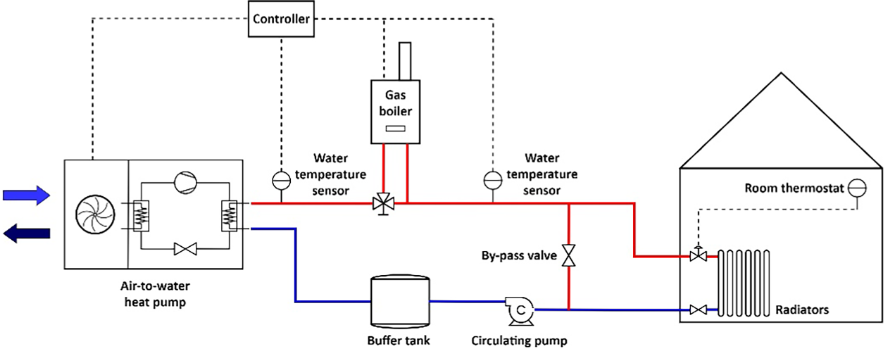
\includegraphics[width=0.85\linewidth]{hhsawhpboiler}
    \caption{\acs{HHS} with an \acs{AWHP} and condensing gas boiler \cite{dongellini_influence_2021}}
    \label{fig:hhsawhpboilerdiagram}
\end{figure}

\citeauthor{heinen_electricity_2016} \cite{heinen_electricity_2016} concluded that \acp{HHS} that use a combination of electricity and gas as the energy source for the heating system can provide the greatest economic benefits when compared to other types of hybrid heating technologies in a combined power-residential heat system. The investment costs of these systems may vary depending on factors such as the size of the system, the specific technology used, and the cost of electricity and gas in the area. However, overall, a \ac{HHPS} that utilises a combination of electricity and gas as the energy source is likely to have the most favourable cost-benefit ratio.

%TODO: Explicitly define what a hybrid heating system is à la Klein and Hutchemann mentioning bivalency, set-point temp, T_biv, show plot, etc. 

\subsection{Operating Modes of \acsp{HHS}}

\graffito{In monovalent systems the entire heat demand, regardless of ambient temperature is supplied with the \HP, but there is hardly any reason to operate in this mode and requires an oversized \HP.}
\subsubsection{Bivalent-Parallel Operation}
\label{subsubsec:biv-parallelop}
In this study, the bivalent-parallel operation paradigm for a \ac{HHS} is used, which is where a controller determines whether to solely run the \HP or conventional gas boiler, or so run them in parallel. \citeauthor{buday_2014} \cite{buday_2014} explains: at temperatures below a certain threshold ($T_\text{cut}$), only the boiler is used, see: domain 1 in \cref{fig:alt-parallel}. Between ($T_\text{cut}$) and a second threshold ($T_\text{biv}$), both the boiler and \HP are used (domain 2). At temperatures above ($T_\text{biv}$), only the \HP is used (domain 3). The second threshold ($T_\text{biv}$) is the temperature at which the \HP can meet the heat demand of the building, and ($T_\text{cut}$) is set to a value such that, when ambient temperatures are above this value, the \HP is ecologically and economically efficient. The optimisation of the bivalent temperature, $T_\text{biv}$, is the crux of this thesis. The cut-off temperature can be calculated using the boiler and \HP efficiency and the \acp{PEF} of the heat sources. 
\begin{figure}[htb]
    \centering
    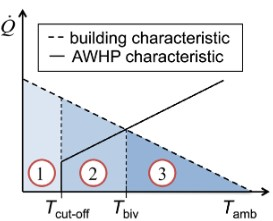
\includegraphics[width=0.4\linewidth]{alt-parallel}
    \caption{Bivalent-parallel operating scheme \cite{klein_numerical_2014}.}
    \label{fig:alt-parallel}
\end{figure}

\subsubsection{Bivalent-Alternative Operation}
In bivalent-alternative operation, the controller has two options in contrast to the three outlined in \cref{subsubsec:biv-parallelop}, either solely use the \HP or solely use the gas boiler \cite{buday_2014}. Below the set bivalent point, the heat demand is entirely provided by the auxiliary heating device, as seen in \cref{fig:bivalentOperationModes}. Above the bivalent temperature, the heat demand is entirely provided by the \HP. This operation places the $T_\text{biv}$ and $T_\text{cut}$ coincident \cite{buday_2014,klein_numerical_2014}. 

\begin{figure}[htb]
    \centering
    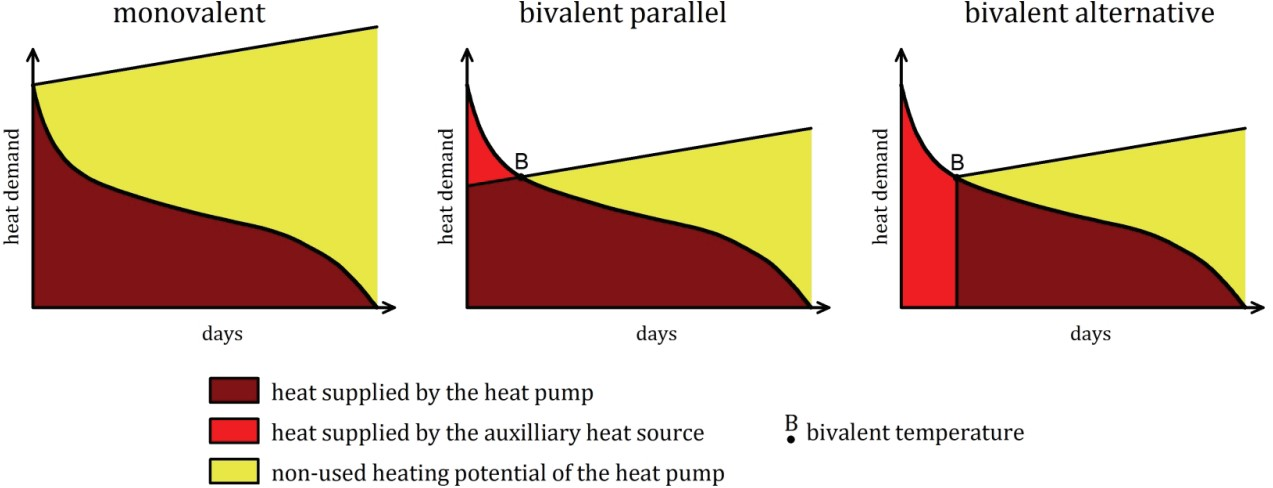
\includegraphics[width=1\linewidth]{bivalentOperationModes}
    \caption[Bivalent operation modes \cite{buday_2014}]{Types of bivalent \ac{HHS} operation modes visualised through heating duration curves \cite{buday_2014}. Note: $T_\text{cut}$ is not clearly shown in this figure.}
    \label{fig:bivalentOperationModes}
\end{figure}

\subsection{Buffer Tank} 
A buffer tank is a medium- to large-sized water vessel used in hydronic heating systems. It provides a large thermal inertia to the heating system-house system, which many small- to medium-sized houses, especially those with poor insulation, lack. Thermal inertia is a desired property of a building as rapid thermal fluctuations in ambient air are less of a concern when it comes to maintaining a comfortable thermal environment indoors. This effect is noticeable in large office/district buildings with high thermal inertias and plays a significant role in heating-capacity selection \cite{owen_ashrae_2009}. Furthermore, a buffer tank provides a ``hydraulic switch'' and allows for heat generation and heat distribution to be in separate loops. This opens up the option to have differing flowrates between the heat generation and heat distribution loops. 

Buffer tanks have been found, when sized correctly and with an appropriate control strategy, to have a positive influence on the efficiency and performance on \acp{HHS} \cite{klein_numerical_2014,roccatello_analysis_2022}. The controller is able to make use of the \HPs ``most profitable working conditions'' thanks to the presence of the buffer \cite{dettorre_economic_2018}. It has been found that when a buffer thank is present in the \HP circuit, \ac{SPF} increases as the size of the \HP decreases \cite{mugnini_variable-load_2021}. \citeauthor{mugnini_variable-load_2021} \cite{mugnini_variable-load_2021} confirmed this for all sizes of \HPs simulated, the smallest buffer tank having a capacity of \SI{200}{\liter}. \citelist{STIEBEL_2012}{organization} \cite{STIEBEL_2012} suggest to size the buffer tank so large as to at least be able to defrost the coils.

\acp{ASHP} can experience negative effects when operated at partial load, such as on-off cycle deterioration. This is caused by losses in the start-up and standby stages, where there is a delay in heating output and power consumption but no heat produced \cite{dongellini_-off_2019}. To prevent these losses and excessive on-off cycles, a buffer tank can be installed in series with the heat pump, providing the hydraulic switch mentioned earlier \cite{bagarella_cycling_2013,dongellini_-off_2019}. In addition to protecting the heat pump from negative effects of partial load operation, the buffer tank also plays a role in maintaining indoor thermal comfort during reverse defrosting, as discussed in \cref{subsec:defrost}.

The larger a buffer tank in volume, the larger its energy storage capacity. However, with a larger volume, and naturally larger cylinder and surface area, comes greater heat loss, which seem to correlate almost linearly \cite{klein_numerical_2014}. This could be justified if other performance factors such as \ac{SPF} or load factor were positively affected to offset this loss in heat, however this does not seem to be the case according to \cite{roccatello_analysis_2022} and \cite{klein_numerical_2014}, which also found only a moderate reduction in on-off cycles with smaller tanks. This is partly to do with the thermal inertia of the building and return temperature controller. 
\citeauthor{klein_numerical_2014} found that the volume of the buffer tank had very limited effect on the system performance. \citeauthor{dongellini_influence_2021} \cite{dongellini_influence_2021} sized their buffer tank just large enough such that the maximum number of on-off cycles was never greater than six per hour,  resulting in a buffer tank with a volume of \SI{79}{\litre}.  This maximum on-off cycle figure was chosen based off their \HP manufacturer guidelines.% Daikin suggest %FIND SUGGESTED MAX NUMBER OF ON-OFF CYCLES FROM DAIKIN.  \cite{dettorre_economic_2018}

\subsection{Frosting and Defrosting} \label{subsec:defrost}
Frosting occurs in \acp{ASHP} in colder ambient temperatures resulting in issues for \HPs. Frost build up depends on the ambient temperature, temperature of the surface in question and relative humidity. For \HPs, a few ranges of temperatures at which frosting occurs has been found in the literature \citeauthor{sandstrom_frosting_2021} \cite{sandstrom_frosting_2021} finding a range of \qtyrange{-15}{6}{\celsius} at a r.h. of $\approx$90\%, while \citeauthor{kropas_experimental_2021} \cite{kropas_experimental_2021} found frost formation to begin when the ambient air temperature was below \SI{3.5}{\celsius} with a r.h. of 88\%. Frosting specifically occurs when the surface temperature of the fins on the air-side heat exchanger component (evaporator) are lower than the freezing point of the of the air. Water droplets start to form and collect on the fins. When the temperatures is below freezing or close to it, the water droplets freeze to the fins and build up a frosting. Frost, unlike snow, which both form from the freezing of water droplets, is not loose and must be scraped off or melted off. It will not \textit{fall off of} a surface like snow might. This layer of frost acts as a layer of insulation and restricts the heat exchanger from transferring heat from the ambient air. Since these fins are typically closely packed, if the layering of frost continues and progressively builds up, the airflow around the fins decreases and so does convective heat transfer to the ambient air, further exacerbating the issue of insulation. All of this is to say that when frosting occurs in \acp{ASHP}, their performance declines severely, from a \ac{COP} circa 3.25 to less than 2 with light- to medium-frosting \cite{di_perna_experimental_2015}. Smaller \HPs tend to be affected to a greater extent than larger capacity \HPs \cite{bee_variable-speed_2016}. \citeauthor{zhang_experimental_2018} \cite{zhang_experimental_2018} found that the temperature of the air and surface of the fins, humidity, velocity of air are the main factors involved in frost formation. 

Many treatments for frosting have been proposed and implemented into products. There is however no golden bullet solution, all of them advantages and disadvantages. Three main solutions are typically used when addressing the issue of frosting in \acp{ASHP}. 
\begin{itemize}
    \item Simple on-off defrosting: the \HP is simply switched off when too much frost has formed on the outdoor component. The performance has been degraded to such a point that it is now economically advantageous to turn off the \HP and wait for the frost to melt away. This however, takes a long time and can negatively affect the thermal comfort of a home if no other heat production is used. The \HP does not use any power during this off-cycle of course, retaining the \ac{COP} of the \HP---although, this may affect the overall system performance if a gas boiler needs to be used to provide the entire heating load of the home.
    \item Reverse cycle defrosting: this method is similar to the first method; the refrigerant is cycled in reverse and hot gas is forced into the heat exchanger. Recall that \HPs and refrigerators differ only in objective. The \HP now treats the outdoors as the ``cold'' sink and begins transferring heat from indoors to outdoors. Intuitively, one can see that this is quite detrimental to the \ac{SPF} of the \HP as the house is being actively cooled by the \HP in order to heat up the outdoor coils and fins to melt away the frost, which in turn causes the auxiliary heater to work even harder to maintain a comfortable indoor temperature. The intention in this method is to melt the frost much quicker than the first method, allowing the \ASHP to begin warming the home once again much earlier than the the simple on-off defrosting method.
    \item Resistive heating: electric resistive heaters are installed on/in the heat exchanger. This method works very well, quickly melting off frost and is a separate heating element to the \HP and therefore does not interrupt the \HPs cycles. Resistive heaters are very expensive to run and negatively affect the \ac{COP} of the \HP.
\end{itemize}

\citeauthor{amer_review_2017} \cite{amer_review_2017} found that the reverse cycling method resulted in a higher average \ac{COP} than the other two methods, over a series of multiple reverse cycle defrostings. Additionally, \citeauthor{bagarella_annual_2016} \cite{bagarella_annual_2016} found that a buffer tank can ensure thermal comfort during reverse cycle defrosting, due to being able to use the stored energy from the buffer tank to melt the frost on the outdoor coils without actively cooling the indoor space due to the inherent decoupling of the heat production and distribution loops created by the buffer tank. \citeauthor{bagarella_annual_2016} \cite{bagarella_annual_2016} agreed with \citeauthor{dong_2012} \cite{dong_2012} that the \textit{defrosting efficiency} of the reverse cycling method is around 60\%. This is the ratio of energy supplied to the coils, to the actual energy transferred to the frost for melting. 

\section{\acsfont{HDD} and Design Temperatures} \label{sec:hddanddesign}
\acp{HDD} is a measure of the difference between the outside temperature and the inside temperature. \acp{HDD} are usually considered over a period of time, be it a month, heating season or entire year. A \textit{base} temperature is chosen, typically around \qtyrange{12}{21}{\celsius} which then determines when it is ``cold'' outside, or can be thought of as being the temperature above which heating is no longer considered to require heating. This base temperature can be chosen at will, and simply depends on what the person/institution deems to be \textit{warm enough}. This measure can be used to quantitatively compare the heating demand of a given house in different locations/climates. The heating requirement of a specific building is directly proportional to the \ac{HDD} \cite{chartered_institution_of_building_services_engineers_environmental_2006}.

To calculate  the \ac{HDD} for a certain day, three equations are used and are displayed from \cref{eq:hdd}. Which equation to use is determined by the interaction between the base temperature and the maximum temperature recorded during that day.  

\begin{align}\label{eq:hdd}
    \text{Degree days} = \begin{cases}
        t_\text{base} - \frac12(t_\text{max} + t_\text{min}), & \text{if } t_\text{max} < t_\text{base}\\
        \frac12(t_\text{base} - t_\text{min}) -\frac14(t_\text{max} -t_\text{base} ), & \text{if } t_\text{base} > \frac12(t_\text{max} + t_\text{min}) \\
        \frac14(t_\text{base} -t_\text{min} ), & \text{if } t_\text{base} <\frac12(t_\text{max} + t_\text{min})
     \end{cases}  
\end{align}

To calculate the Monthly degree days however, only the first of the three equations in \cref{eq:hdd} is made use of. This total is found by summing the daily temperatures differences and can be seen in \cref{eq:mdd}.
\begin{equation}
    \text{Monthly degree days} = \displaystyle\sum_\text{month} \left[t_\text{base} - \frac12(t_\text{max} + t_\text{min})\right] \label{eq:mdd}
\end{equation}

\citetitle{chartered_institution_of_building_services_engineers_environmental_2006} has chosen a base temperature of \SI{15.5}{\celsius}. \citetitle{owen_ashrae_2009} used a base temperature of \SI{18.3}{\celsius} and determined an annual \ac{HDD} of \SI{3135}{\celsius\day} for Dublin Airport, IE, N\ang{53;26;} W\ang{06;15;}. Using the online tool \texttt{Degree Days.Net} \cite{degreedays} with a base temperature of \SI{15.5}{\celsius}, a \ac{HDD} figure of \SI{2072.3}{\celsius\day} was obtained for the same location.  

Design temperatures are a measure how many hours/days a specified condition is exceeded. In the case of a heating design temperature, this would indicate how many days of the year or heating season are spent below a given temperature. \citetitle{owen_ashrae_2009} \cite{owen_ashrae_2009} notes that this measure does not give an indication of the frequency or duration of these events, only a cumulative result is returned. According to \citetitle{owen_ashrae_2009} \cite{owen_ashrae_2009}, the 99.6\% design temperature in Dublin Airport is \SI{-1.9}{\celsius} while the 99.0\% design temperature is \SI{-0.7}{\celsius}. Traditionally, conventional gas boilers or resistive heaters were sized to design temperatures, meaning, for a chosen design temperature percentile (e.g., 99.0\%), the heater could heat the building to thermally comfortable levels for 99\% of the year, however during the 1\% temperature lows, the heater would not be adequate. This calculates to the heater being undersized for $\sim$35 hours of the year. \graffito{$365\times24=\SI{8760}{\hour} \Rightarrow 99.0\%\text{-ile} = 8760(100-99.0) = \qty{87.6}{\hour}$ }

In monovalent systems, the \HP is sized in such a way as to be able to provided the entire heating load for a building at design conditions. This results in the \HP being positively over-dimensioned for the task \cite{klein_numerical_2014}. An oversized heating system would be very inefficient due to frequent on-off cycling \cite{blackman_study_2019}, which also results in rapid degradation of heating system components. Oversized heating systems also result in potentially uncomfortable indoor temperatures as rooms are unequally heated \cite{rauschkolb_cost-optimal_2020}. Finally, oversized systems have higher maintenance costs and significantly higher initial investment costs.\graffito{for the purposes of the simulation(s) concerning this thesis, the 0.4 percentile, and any cooling-nessecary-temperatures for that matter, are not of concern as cooling is out of scope.}

The  concept of a \textit{design-day} can be used to design heating configurations for homes, especially when performing numerical simulations on a model of the system \cite{rauschkolb_cost-optimal_2020}.  A design-day file is a special weather file created with design conditions in mind. Based on the design temperature parameter, \citelist{owen_ashrae_2009}{institution} lays out a procedure to generate a 24-hour weather profile. These profiles represent the 0.4\% to 99.6\% extremes experienced for a particular location \cite{owen_ashrae_2009}. This weather data is used in simulations to determine the minimum size for a heater required for a house (for these particular percentiles of course). 

The ``heating duration curve'' can be devised for a specific climate and a specific \HP where a curve is plotted on a chart with heating load [\unit{\kilo\watt\per\hour}] against number of hours the heating load is equal to or above a selected percentage of design load \cite{todorovic_achieving_2019}. For example, as illustrated in \cref{fig:heatingloaddurationcurve}, the blue line indicates 50\% design load, and lands around 1300 hours on the $x$-axis. This means that for 1300 hours of the year/heating season, the heating load of the building is 50\% of the design (or max) load. The balance point marked by the yellow circle is the point at which the \HP is not longer able to provide the entire heating load required by the building. To the left of this point, the gas boiler will need to provide the remaining heat capacity to maintain a comfortable indoor temperature. If the \ac{AWHP} size is increased, this balance point moves to the left, as the \HP can provide the entire heating envelope of the building at lower temperatures. Of course, for the sake of the diagram, the curves and lines in this figure are arbitrary (e.g., \ac{AWHP} performance is not linear with outdoor temperature, and by proxy, heating load), but it illustrates how a \HP may be sized to 60\% of the design load of a building.

\begin{figure}[htb]
    \centering
    \import{tikz/}{heatingDurationCurve.tex}
    \caption{Example heating duration curve highlighting bivalent point. It shows the cumulative number of hours that a heating system needs to operate at various levels of heat demand}
    \label{fig:heatingloaddurationcurve}
\end{figure}

All of this is to say that there are many methods of determining and comparing the heating load of a building for a given climate, with which heating devices may be sized to in order to be able to (almost always) have the capacity to heat a building. A \ac{HHS} is unique in that it is composed of two heating devices. The boiler, as stated before, is sized to a certain high-percentage design condition. This may be defined by the user/homeowner, convention, or by some set of standards set by a governing body (e.g., ASHRAE), and is typically a value in the region of 95\% to 99.7\%. On account of this, the \ac{AWHP} can be sized smaller than compared to if it were the sole heating device.

\section{Primary Energy}\label{sec:primaryenergy}
\ac{PE} is a term used in the fields of energy statistics and energetics. Sources of \ac{PE} are those which have not been interfered with by humans, in other words, are the natural form of energy and are unprocessed. \ac{PE} sources include: oil, natural gas, sunlight, wind, etc. \ac{PE} stands in contrast to secondary energy, which can be thought of as the carrier of energy, which most commonly happens to be electricity, but can also be liquid forms of energy (e.g., diesel/petrol, ), hydrogen fuel cells or (waste) heat. Following from \ac{PE}, is \ac{PEF} which connects \ac{PE} to final energy, it is a measure of how much energy in total is required to produce a unit of \textit{usable} energy \cite{nowak_2018}. The \ac{PEF} is used to evaluate the environmental impact of a system by considering the primary energy consumption, which includes the energy required to produce and distribute the energy source, such as the energy used to extract and transport fossil fuels. For example, a hydroelectric power plant with a \ac{PEF} of 1, means that the energy used to generate electricity is equal to the energy consumed. On the other hand, a coal-fired power plant with a \ac{PEF} of 2.5, means that 2.5 units of \ac{PE} are consumed to generate 1 unit of electricity. Therefore, hydroelectric power plants are considered more environmentally friendly than coal-fired power plants. \cite{bianco_estimation_2017} found that with a suitably high diffusion of \ac{RES} in an electrical grid, significant \ac{PES} can be obtained through the use of \HPs for space heating and can overall promote energy savings in buildings, in turn reducing $\text{CO}_2$ emissions \cite{nowak_2018}.   

\cref{fig:PEtoFinalSankey} is a Sankey diagram which breaks down the flow of energy in Ireland in 2020 from \ac{PE} on the left by fuel type, and final energy on the left, by sector. It also highlights the energy losses associated with energy production and transmission. It requires energy to convert natural gas or oil to electricity, while energy losses corresponding to renewable energy production are dismissed, as the energy source is of course \textit{free}. 

\begin{figure}[htb]
    \centering
    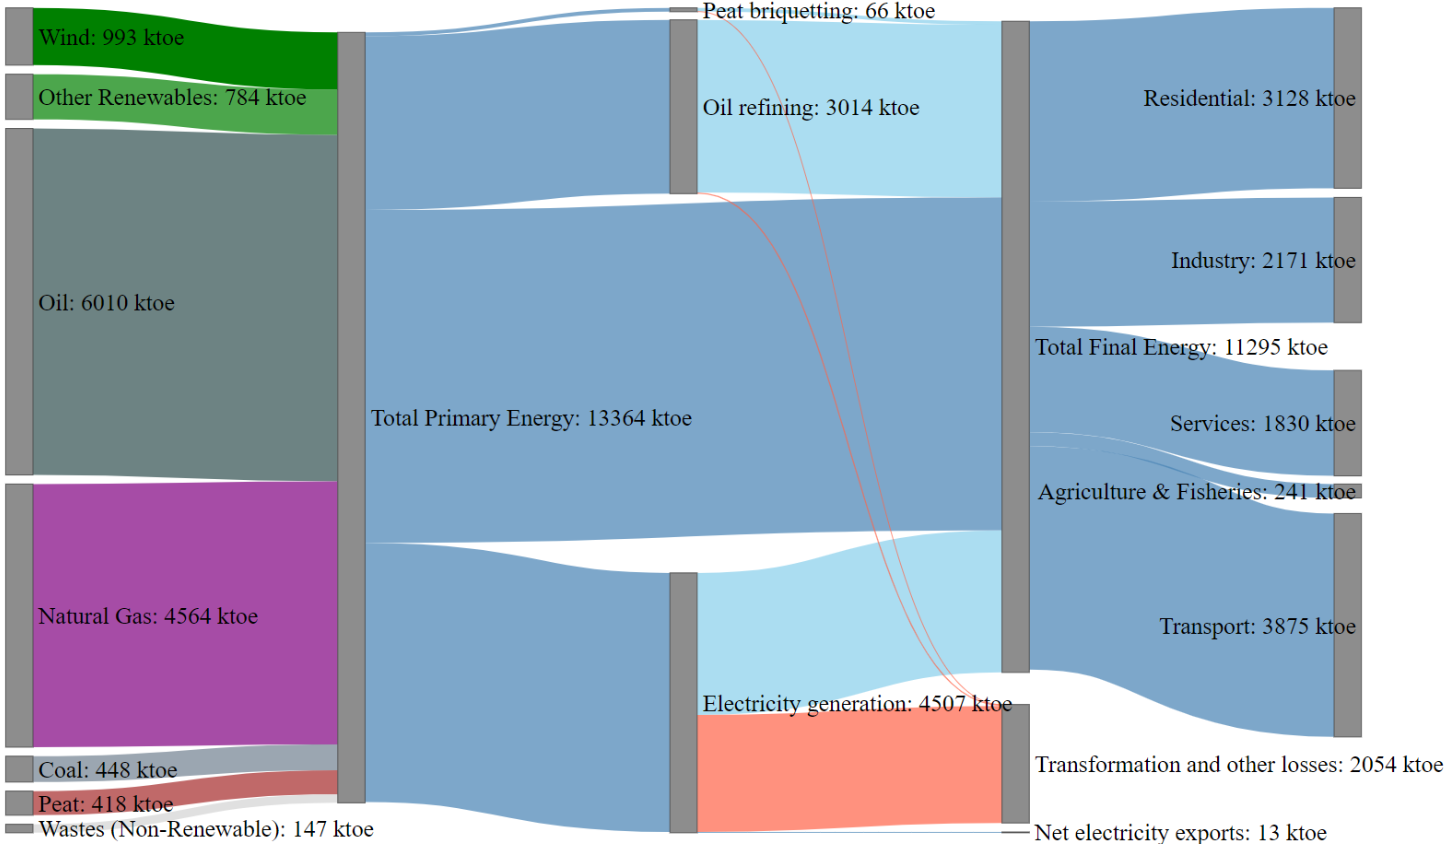
\includegraphics[width=0.85\linewidth]{primaryEnergyToFinalEnergySankey}
    \caption[\acs{PE} breakdown by fuel type and sector]{Sankey diagram showing \acs{PE} by fuel type on left and final energy by sector on right \cite{seai_energy_2021}.}
    \label{fig:PEtoFinalSankey}
\end{figure}

\ac{PES} is difference between the amount of energy consumed by the original device (whatever it may be) and the amount of energy consumed by the new device. In relation to this thesis, it will be taken to be the savings of the new heat generation system compared to the old system (conventional gas boiler as sole heat production). Knowledge of the \ac{PEF}, \ac{PES} and the make-up of the fuel types and shares in the \ac{PE}, i.e., the \ac{RES}, can indicate how much $\text{CO}_2$ is consumed at any instance with a heating system \cite{bianco_estimation_2017}, and is the foundation of the techno-ecological model of this thesis. 

The \ac{RES} of an electrical grid refers to the proportion of electricity generated from renewable energy sources, such as solar, wind, hydro, geothermal, and biomass, compared to the total electricity generation. It is a measure of how much of the electricity being consumed by a country or region is coming from renewable sources. For example, if an electrical grid generates \qty{50}{\giga\watt} of electricity and \qty{20}{\giga\watt}  of it is generated from renewable sources, the \ac{RES} of that grid is said to be 40\%.

The \ac{RES} is an important metric to measure the progress towards decarbonization and the reduction of greenhouse gas emissions in the energy sector. Governments and international organisations have set targets for the increasing share of renewable energy in the electricity mix as a means of reducing the dependence on fossil fuels and reducing the emissions of greenhouse gases \cite{sachs2022sustainable}. Knowing the \ac{RES} of an electrical grid can also help understand the potential for further integration of renewable energy sources and the necessary investments in infrastructure and technology to achieve the goals set by the government or international organizations. In addition, the \ac{RES} of an electrical grid can also impact the stability of the grid and the integration costs, it is important for grid operators and policy makers to consider this metric when planning for future energy systems \cite{sachs2022sustainable}.


\section{Electrification of Heating} \label{sec:elecheating}
The EU has now for a number of years been pushing for the electrification of heating throughout the union. This has been identified as a clear means to achieve decarbonisation goals, as concerns over global warming become greater. As noted in \cref{sec:context}, the residential sector contributes 27\% of the final energy consumption, while residential domestic water production and space heating contributes to 80\% of that. In Ireland, residential heating accounted for 53\% of $\text{CO}_2$ emissions from heating. However, across all sectors, heating and cooling are responsible for half of all final energy consumption in the EU \cite{an2016strategy}. Therefore, it is clearly evident that decarbonisation of the heating/cooling sector is vital to a) reaching EU targets of lowering $\text{CO}_2$ emissions and b) improving air quality and the reduction of harmful emissions \cite{epri2018us}. Although, switching to electrically driven heating systems does not automatically or inherently reduce the carbon emissions, merely, it changes the source of the energy; the electricity must also be decarbonised for this to be the case. 

\citeauthor{seai_energy_2021} \cite{seai_energy_2021} carried out a comprehensive study on the Irish electrical grid performance as it relates to renewable energy sources and to heating/cooling. According to the report: the share renewable energy to that of the the total energy used in 2020 was 13.5\% (having missed the EU target of 16\%); the share of renewable energy used specifically in heating/cooling was just 6.3\%, its target having been 12\%; energy from renewable sources grew by 8.9\% over the previous year, and the total installed wind energy capacity grew by 4.1\%, from \SI{4130}{\mega\watt} to \SI{4310}{\mega\watt} (in the Republic). Overall, the residential energy $\text{CO}_2$ emission has trending downwards over the past decade and a half, falling by 25\% since 2005, and the $\text{CO}_2$ intensity of electricity generation is half of its value in 2005, standing at \SI{300}{\gram\per\kWh}. \graffito{Emission intensity is a measure of how much $\text{CO}_2$ is released per unit of energy produced}These are good signs for the electrification of heating, because in order for the electrification of heating to result in a decarbonising of heating, the electricity production must at least have a lower emission intensity compared to if no electrification process were to take place, but ideally have the prospects of becoming a very low/zero $\text{CO}_2$ intensity matter.

\section{Controllers and Control Theory} \label{sec:controltheory}
Control theory is concerned with the control of dynamic systems with with a desired goal in mind, which is called the reference. A controller manipulates the inputs to a system, usually denoted $u$, in such a way as to alter the output variables or states, $y$, of the system to follow a given reference. Disturbances, $d$, to a system are expected, yet unforeseen inputs to a system which may significantly alter the outputs state.  There are two main types of controller, feed-forward, and feedback controllers \cite{Franklin2014}.

A feed-forward controller, also known as an open loop controller, controls the system without knowing the current state of the system \cite{vries_learning_2000}. This is possible if disturbances are either eliminated, or wholly understood and accounted for.\graffito{However, they would they no longer qualify as disturbances, and would simply be considered as inputs, but that is by the by.} Complete knowledge of the dynamics of the system being controlled would be required and captured by a mathematical model, either by physics and first principles, or by system identification (a model is fitted to data) \cite{vries_learning_2000}. The dynamics of the system are inverted by the controller and fed to the system as inputs. Any error in the inversion process results in undesired system states. 

Feedback controllers, also known as closed loop controllers are a \textit{much} more common form of controller. The current system state is known to the controller, and the reference and current state information is used to determine the appropriate control inputs. In doing so, a feedback controller inherently changes the dynamics of a system. Feedback controllers usually make systems more stable, however, there is the possibility of making systems less stable and even unstable through controllers \cite{Franklin2014}. There are many types of feedback controllers, the most common and well understood kind being a linear feedback controller called a \ac{PID} controller, or just a \ac{PID}. Linear controllers assume the general behaviours of the system to be linear. Although, even if the dynamics of system are not, in fact, linear, a \ac{PID} will still likely be able to control the system appropriately and reach the reference state \cite{Rames_2012}.

In a \ac{HHS}, controllers are used to manage the operation of the different heating technologies and ensure that they are used in the most efficient and effective way possible \cite{di_perna_experimental_2015,bagarella_annual_2016,roccatello_analysis_2022,demirezen_feasibility_2021,mugnini_variable-load_2021,bianco_estimation_2017}. The controllers in a \ac{HHS} are typically responsible for a number of tasks, including monitoring the temperature inside and outside the building, determining the best heating technology to use based on the current conditions, and controlling the operation of the heating technologies to maintain a comfortable and consistent temperature.

For example, when the outside temperature is cold, the controller may determine that it is most efficient to use the gas furnace to heat the building. When the outside temperature is mild, the controller may determine that it is more efficient to use the \HP, which uses less energy than the gas furnace. Very advanced controllers may also use predictive algorithms and weather forecasts to anticipate changes in temperature and adjust the heating system accordingly by storing a lot of heat in the buffer tank during a warm period right before a cold period \cite{demirezen_feasibility_2021}.


\begin{figure}[htb]
    \centering
    \begin{subfigure}[t]{1\textwidth}
        \centering
        \import{tikz/}{controller.tex}
        \caption{Basic feed-forward/feedback hybrid controller \cite{elprofessor_tikz_2019}}
        \label{fig:controller}
    \end{subfigure}
    \hfill
    \begin{subfigure}[t]{0.7\textwidth}
        \centering
        \import{tikz/}{pid.tex}
        \caption{The workings of a \acs{PID} controller \cite{mmm_left_2012}}
        \label{fig:pid}
    \end{subfigure}
    \caption{Representative block diagrams of a hybrid controller system and a \acs{PID} controller}
    \label{fig:visualisations}
\end{figure}

\subsection{\acs{PID} Controllers}
\ac{PID} controllers are a type of feedback control system that are commonly used in a wide variety of systems to maintain a desired output or setpoint. The acronym refers to the three components of the control algorithm used by the controller. \ac{PID} controllers work by continuously calculating an error value that represents the difference between the desired setpoint and the current output of the system. \citeauthor{Rames_2012} \cite{Rames_2012} explains that this error value is then used to calculate and apply a correction to the system, based on the three components of the \ac{PID} algorithm:
\begin{itemize}
    \item The proportional component applies a correction proportional to the error value. This allows the controller to quickly respond to large errors and make large corrections.
    \item The integral component applies a correction based on the accumulated error over time. This helps to eliminate steady-state errors and ensure that the system eventually reaches the desired setpoint.
    \item The derivative component applies a correction based on the rate of change of the error. This helps to dampen the system's response and prevent overshoot and oscillation.  
\end{itemize}


\ac{PID} controllers are used in a wide variety of systems, including mechanical systems like motors and actuators, temperature control systems, and chemical process control systems. They are often preferred over other control algorithms because they are relatively simple to implement and can provide stable and accurate control of the output of the system.

\subsection{Noise and Error}
Noise and error are common sources of problems in control systems. Noise refers to random variations in the output of the system that are not caused by the control signal, while error refers to the difference between the desired setpoint and the actual output of the system \cite{Rames_2012}. Noise and error can have a number of adverse effects on the performance of a control system, including reduced accuracy and stability, as well as increased oscillation and overshoot. To deal with noise and error in control systems, a number of different approaches can be used. One approach is to use a filter to remove noise from the output of the system signal. This can be done using a low-pass filter, which removes high-frequency noise, or a high-pass filter, which removes low-frequency noise \cite{Franklin2014}. Another approach is to use a model-based control algorithm, which uses a mathematical model of the system to predict the output of the system and apply appropriate control signals. This can help to reduce the effects of noise and error by using the model to compensate for them . Furthermore, another approach is to use a robust control algorithm, which is designed to be resistant to the effects of noise and error. Robust control algorithms typically use a combination of feedback and feed-forward control, as well as advanced control techniques like gain scheduling and optimization, to achieve robust performance in the presence of noise and error.

\section{Verification \& Validation of Model} \label{sec:verifyandvalid}
Verification and validation are two important processes that are used to assess the credibility and reliability of a simulation model. While these terms are often used interchangeably in common parlance, they have distinct meanings and serve different purposes.

Verification is the process of ensuring that a simulation model is implemented correctly and accurately represents the underlying mathematical equations, assumptions, and physical phenomena. Verification ensures that the simulation code is free from coding errors and that the numerical algorithms are implemented correctly, and confirms whether the model behaves as the modeller expects. This process involves checking the model against analytical solutions or known results and comparing the simulation output with the expected results \cite{judkoff_methodology_2008}.

Validation, on the other hand, is the process of determining whether a simulation model accurately represents the real-world system it is intended to simulate. Validation involves comparing the model output to real-world observations and data to assess the accuracy of the model in predicting system behaviour. This process also involves assessing the sensitivity of the model to input parameters and assumptions. The underlying values of the model (e.g., insulation thickness, floor tile conductivity, etc.) are altered and calibrated to fit the real-world data \cite{ruiz_validation_2017}.

\acp{BEM} must undergo verification and validation due to various sources of uncertainty arising naturally as a result of converting a real-life problem to a mathematical model to a numerical model. Four sources of uncertainty particular to \acp{BEM} are identified by \cite{coakley_review_2014,DEWIT2002951} as: 
\begin{itemize}
    \item Specification uncertainty arises from incomplete or inaccurate specifications of the building or systems being modelled. 
    \item Modelling uncertainty results from simplifications and assumptions of complex physical processes. 
    \item Numerical uncertainty is introduced during the discretisation and simulation of the model. 
    \item Scenario uncertainty comes from external conditions imposed on the building, such as outdoor climate conditions and occupant behaviour.
\end{itemize}


\subsection{Validation} \label{subsec:validation}
The validation process of a \ac{BEM} is a crucial step in ensuring that the model accurately predicts the energy performance of the building. Calibrating a building involves adjusting the energy model to better reflect reality \cite{coakley_review_2014,farhang2012monitoring}. This is done by comparing measured data to simulated data, and performing an uncertainty analysis to determine how well they match. Although real and measured data can be similar, there may still be errors in the simulation \cite{ashrae_guideline_project_committee_14_ashrae_2014}. Various factors, such as weather \cite{lucas2019methodology} or occupancy, can introduce uncertainty, along with envelope uncertainties. The \citetitle{ashrae_guideline_project_committee_14_ashrae_2014} \cite{ashrae_guideline_project_committee_14_ashrae_2014} provides a comprehensive framework for validating \acp{BEM}. This guideline outlines a step-by-step process for validating the simulation model and includes criteria for evaluating the accuracy of the model. The validation process involves comparing the model results with actual building energy consumption data and performing statistical analysis to determine the level of accuracy. In the validation process used in this thesis, three statistical tools or indices are employed to evaluate the accuracy of the simulation model in this thesis. The first two are suggested by \citelist{owen_ashrae_2009}{institution} while the last is used as its properties are distinct from the first two and provides a useful measure of absolute error.


\ac{CVRMSE} is a statistical tool used to determine the degree of error between the simulated and actual data and is a commonly used tool in the validation process of \acp{BEM} because it takes into account the variability in the actual data \cite{ashrae_guideline_project_committee_14_ashrae_2014}. It calculates the \ac{RMSE} as a percentage of the mean of the actual data, which makes it a useful metric for evaluating the accuracy of the model across a range of operating conditions. A lower \ac{CVRMSE} value indicates that the model is a better predictor of the actual building energy performance. The \ac{CVRMSE} tool is particularly useful when comparing the performance of different models or when assessing the impact of different input parameters on the accuracy of the model. \citeauthor{coakley_review_2014} \cite{coakley_review_2014} said: ``[\ac{CVRMSE}] allows one to determine how well a model fits the data by capturing offsetting errors between measured and simulated data. It does not suffer from the cancellation effect.''. The formula for \ac{CVRMSE} is given by \cref{eq:cvrmse}.

\begin{equation}
    \acsfont{\operatorname{CV(RMSE)}} = \frac{100}{\bar{Y}} \sqrt{\frac{\sum_{i=1}^N(Y_i - \hat{Y}_i)^2}{N-p}} = \frac{\operatorname{RMSE}}{\bar{Y}}  \label{eq:cvrmse}
\end{equation}

\ac{NMBE} is another statistical tool used in the validation process, measuring the bias of the model. It provides a measure of the difference between the mean of the simulated and actual data as a percentage of the actual data \cite{ashrae_guideline_project_committee_14_ashrae_2014}. A zero \ac{NMBE} value indicates that the model is unbiased, while a positive or negative \ac{NMBE} value indicates overestimation or underestimation, respectively. The  \ac{NMBE} tool is useful in identifying systematic errors in the model, which can occur due to incorrect model assumptions, data input errors, or other issues. It helps to identify the direction and magnitude of the bias, which is important for developing strategies to improve the accuracy of the model. The formula for \ac{NMBE} is given by \cref{eq:nmbe}.

\begin{equation}
    \acsfont{\operatorname{NMBE}} = \frac{100}{\bar{Y}} \frac{\sum_{i=1}^N(Y_i - \hat{Y}_i)}{N-p} \label{eq:nmbe}
\end{equation}

\ac{SMAPE}, first proposed by \citeauthor{MAKRIDAKIS1993527} \cite{MAKRIDAKIS1993527} and approved by many \cite{tofallis_better_2015,khendek_system_2018,kim_new_2016}, is a statistical tool that measures the absolute percentage difference between the simulated and actual data. Unlike the previous two tools, \ac{SMAPE} is symmetric and thus gives equal weight to overestimation and underestimation. A lower \ac{SMAPE} value indicates higher model accuracy. It is an extension of the MAPE method which has the flaw of being asymmetric in its treatment of over- and underprediction of the actual value, overpredictions being penalised harder than underpredictions. There are three common definitions of \ac{SMAPE}, each with different properties, however, this thesis chooses to use the definition which outputs values as a percentage error between 0\% and 100\% as this is most easily interpretable and comparable. The formula for \ac{SMAPE} is given by \cref{eq:smape}.

\begin{equation}
    \acsfont{\operatorname{SMAPE}} = \frac{100}{N} \sum_{i=1}^N\frac{|Y_i - \hat{Y}_i|}{|\hat{Y}_i|+|Y_i|} \label{eq:smape}
\end{equation}

\citetitle{ashrae_guideline_project_committee_14_ashrae_2014} \cite{ashrae_guideline_project_committee_14_ashrae_2014} suggest different tolerances for data calibrated by monthly or by hourly data for the \ac{CVRMSE} and \ac{NMBE} statistical methods. \citelist{owen_ashrae_2009}{institution} suggests tolerances of <15\% for \ac{CVRMSE} and $\pm$5\% for \ac{NMBE} for comparisons done by a monthly basis. A simulation is said have high levels of model prediction performance if absolute percentage error values outputted by \ac{SMAPE} are less than 20\% and great levels if less than 10\%. 


\section{Conclusion}
In this literature review, the fundamental concepts behind the operating principles of \HPs was described, the dynamics of \acp{HHS} were described, the effects of the different operating modes and physical phenomena were detailed, and Heating-system design was studied. The reasoning behind (future and current) policies pushing for \HP adoption were explained along with the basics of control theory were. Finally, the verification and validation of numerical simulation models was discussed along with the statistical models to be used later on in the thesis. The literature surrounding \acp{HHS} and \HPs is vast, however, perhaps the most succinct---and perhaps discouraging---statement/expression in the literature is: ``numerical findings are generally idiosyncratic to geographical contexts, time horizons as well as assumptions on costs, policies, and technology availability'' \cite{bloess_power--heat_2018}\ldots\ \citeauthor{rauschkolb_cost-optimal_2020} \cite{rauschkolb_cost-optimal_2020} explain how small variations in the price of natural gas can shift fossil fuel-only systems from being the best economic choice to the worst. 

After the literature review, it was found that there is a significant gap in research regarding the bivalent operation temperature window and its impact on \acs{HHPS}. Very few papers have explored this topic, making it a crucial area of investigation. Additionally, the few studies available have primarily focused on continental climates and not on the temperate oceanic climate. 

